\tikzstyle{image} = [rectangle, draw, fill=blue!20, 
    text width=1.5cm, text centered, minimum height=1cm]
\tikzstyle{imaged} = [rectangle, draw, fill=blue!20, 
    text width=.74cm, text centered, minimum height=.45cm]
\tikzstyle{imagedd} = [rectangle, draw, fill=blue!20, 
    text width=.3cm, text centered, minimum height=.15cm]
%
\tikzstyle{orpi} = [rectangle, draw, fill=orange!40,
    text width=2cm, text centered, rounded corners, minimum height=1cm]
%
\tikzstyle{pimage} = [rectangle, draw, fill=red!20, 
    text width=1.5cm, text centered, minimum height=1cm]
\tikzstyle{pimaged} = [rectangle, draw, fill=red!20, 
    text width=.74cm, text centered, minimum height=.45cm]
\tikzstyle{pimagedd} = [rectangle, draw, fill=red!20, 
    text width=.3cm, text centered, minimum height=.15cm]
%
\tikzstyle{aimage} = [rectangle, draw, fill=green!20, 
    text width=1.5cm, text centered, minimum height=1cm]
\tikzstyle{aimaged} = [rectangle, draw, fill=green!20, 
    text width=.74cm, text centered, minimum height=.45cm]
\tikzstyle{aimagedd} = [rectangle, draw, fill=green!20, 
    text width=.3cm, text centered, minimum height=.15cm]
%
\tikzstyle{cnn} = [rectangle, draw, fill=orange!40,
    text width=2cm, text centered, rounded corners, minimum height=1cm]
\tikzstyle{vector10} = [rectangle, draw, fill=gray!40, 
    text width=1.5cm, text centered, rounded corners, minimum height=1cm]
\tikzstyle{vector1} = [rectangle, draw, fill=gray!20, 
    text width=1.5cm, text centered, rounded corners, minimum height=1cm]
\tikzstyle{svm} = [rectangle, draw, fill=purple!20, 
    text width=1.5cm, text centered, rounded corners, minimum height=1cm]
\tikzstyle{output} = [rectangle, fill=white!0,
    text width=4cm, text centered, rounded corners, minimum height=1cm]
\tikzstyle{labm} = [rectangle, text width=2cm, 
	text centered, minimum height=1cm]
\tikzstyle{line} = [draw, -latex']
\def\elwi{2cm}
\def\I{
\resizebox{\elwi}{!}{
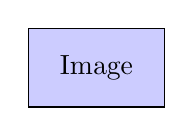
\begin{tikzpicture}
	\node [image] (a) at (0,0) {Image};
\end{tikzpicture}
} }
\def\Id{
\resizebox{\elwi}{!}{
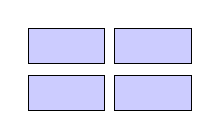
\begin{tikzpicture}
	\node [imaged] (ba) at (-4,.3) {};
	\node [imaged] (bb) at (-2.9,-.3) {};
	\node [imaged] (bc) at (-4,-.3) {};
	\node [imaged] (bd) at (-2.9,.3) {};
\end{tikzpicture}
} }
\def\Idd{
\resizebox{\elwi}{!}{
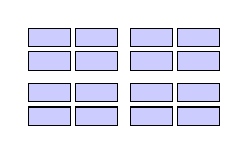
\begin{tikzpicture}
	\node [imagedd] (caa) at (2.3,.5) {};
	\node [imagedd] (cab) at (2.3,.2) {};
	\node [imagedd] (cac) at (1.7,.5) {};
	\node [imagedd] (cad) at (1.7,.2) {};
	%
	\node [imagedd] (cba) at (3,.5) {};
	\node [imagedd] (cbd) at (3,.2) {};
	\node [imagedd] (cbc) at (3.6,.5) {};
	\node [imagedd] (cbd) at (3.6,.2) {};
	%
	\node [imagedd] (cca) at (2.3,-.5) {};
	\node [imagedd] (ccb) at (2.3,-.2) {};
	\node [imagedd] (ccc) at (1.7,-.5) {};
	\node [imagedd] (ccd) at (1.7,-.2) {};
	%
	\node [imagedd] (cda) at (3,-.5) {};
	\node [imagedd] (cdb) at (3,-.2) {};
	\node [imagedd] (cdc) at (3.6,-.5) {};
	\node [imagedd] (cdd) at (3.6,-.2) {};
\end{tikzpicture}
} }
\def\ori{
\resizebox{\elwi}{!}{
\begin{tikzpicture}
	\node [orpi] (p) at (0.0) {Original\\pipeline};
\end{tikzpicture}
} }
\def\red{
\resizebox{\elwi}{!}{
\begin{tikzpicture}
	\node [pimage] (p) at (0.0) {Plastic};
\end{tikzpicture}
} }
\def\Rd{
\resizebox{\elwi}{!}{
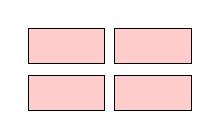
\begin{tikzpicture}
	\node [pimaged] (ba) at (-4,.3) {};
	\node [pimaged] (bb) at (-2.9,-.3) {};
	\node [pimaged] (bc) at (-4,-.3) {};
	\node [pimaged] (bd) at (-2.9,.3) {};
\end{tikzpicture}
} }
\def\Rdd{
\resizebox{\elwi}{!}{
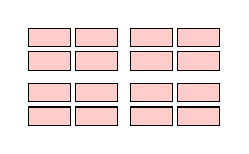
\begin{tikzpicture}
	\node [pimagedd] (caa) at (2.3,.5) {};
	\node [pimagedd] (cab) at (2.3,.2) {};
	\node [pimagedd] (cac) at (1.7,.5) {};
	\node [pimagedd] (cad) at (1.7,.2) {};
	%
	\node [pimagedd] (cba) at (3,.5) {};
	\node [pimagedd] (cbd) at (3,.2) {};
	\node [pimagedd] (cbc) at (3.6,.5) {};
	\node [pimagedd] (cbd) at (3.6,.2) {};
	%
	\node [pimagedd] (cca) at (2.3,-.5) {};
	\node [pimagedd] (ccb) at (2.3,-.2) {};
	\node [pimagedd] (ccc) at (1.7,-.5) {};
	\node [pimagedd] (ccd) at (1.7,-.2) {};
	%
	\node [pimagedd] (cda) at (3,-.5) {};
	\node [pimagedd] (cdb) at (3,-.2) {};
	\node [pimagedd] (cdc) at (3.6,-.5) {};
	\node [pimagedd] (cdd) at (3.6,-.2) {};
\end{tikzpicture}
} }
\def\gre{
\resizebox{\elwi}{!}{
\begin{tikzpicture}
	\node [aimage] (p) at (0.0) {Animals};
\end{tikzpicture}
} }
\def\Gd{
\resizebox{\elwi}{!}{
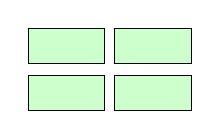
\begin{tikzpicture}
	\node [aimaged] (b1) at (-4,.3) {};
	\node [aimaged] (b2) at (-2.9,-.3) {};
	\node [aimaged] (b3) at (-4,-.3) {};
	\node [aimaged] (b4) at (-2.9,.3) {};
\end{tikzpicture}
} }
\def\Gdd{
\resizebox{\elwi}{!}{
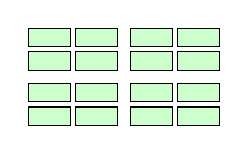
\begin{tikzpicture}
	\node [aimagedd] (caa) at (2.3,.5) {};
	\node [aimagedd] (cab) at (2.3,.2) {};
	\node [aimagedd] (cac) at (1.7,.5) {};
	\node [aimagedd] (cad) at (1.7,.2) {};
	%
	\node [aimagedd] (cba) at (3,.5) {};
	\node [aimagedd] (cbd) at (3,.2) {};
	\node [aimagedd] (cbc) at (3.6,.5) {};
	\node [aimagedd] (cbd) at (3.6,.2) {};
	%
	\node [aimagedd] (cca) at (2.3,-.5) {};
	\node [aimagedd] (ccb) at (2.3,-.2) {};
	\node [aimagedd] (ccc) at (1.7,-.5) {};
	\node [aimagedd] (ccd) at (1.7,-.2) {};
	%
	\node [aimagedd] (cda) at (3,-.5) {};
	\node [aimagedd] (cdb) at (3,-.2) {};
	\node [aimagedd] (cdc) at (3.6,-.5) {};
	\node [aimagedd] (cdd) at (3.6,-.2) {};
\end{tikzpicture}
} }
\def\Pla{
\resizebox{\elwi}{!}{
\includegraphics{images/segment/253_01__plastic__.png}
%\begin{tikzpicture}
%	\node [orpi] (p) at (0.0) {Original\\Pipeline};
%\end{tikzpicture}
} }
\def\Ani{
\resizebox{\elwi}{!}{
\includegraphics{images/segment/253_01__animals__.png}
%\begin{tikzpicture}
%	\node [orpi] (p) at (0.0) {Original\\Pipeline};
%\end{tikzpicture}
} }
\def\mdo{
\resizebox{\elwi}{!}{
\begin{tikzpicture}
	\node [labm] (p) at (0.0) {...};
\end{tikzpicture}
} }
\centerline{
\begin{minipage}{\widefigwidth}
\resizebox{\textwidth}{!}{
\xymatrix{
\I \ar[r]^{devide} \ar[d]^{\times2^0}& \Id \ar[r]^{devide} \ar[d]^{\times2^1}& ... \ar[r]^{devide} \ar[d]& \Idd \ar[d]^{\times2^d}& \\
\ori \ar[d]& \ori \ar[d]& \mdo \ar[d]& \ori \ar[d]& \\
\red \ar[r]^{+}& \Rd \ar[r]^{+}& \mdo \ar[r]^{+}& \Rdd \ar[r]^{=}& \Pla\\
\gre \ar[r]^{+}& \Gd \ar[r]^{+}& \mdo \ar[r]^{+}& \Gdd \ar[r]^{=}& \Ani\\
}
}
\end{minipage}
}
